\chapter{The Brouwer fixed point theorem}
\section{The hex game}
A \emph{hex board}\define{hex!board}\define{board!hex} is a diamond of regular hexagonal tiles, with an equal number of hexagons on each side.
\begin{center}
\tiny
\includegraphics[width=\textwidth]{hex-board}
\par\noindent{}Exhibit made by Massami Takahashi, photo by Rodrigo.Argenton.
Creative Commons Attribution-Share Alike 4.0 International license.
\end{center}
A game of \emph{hex}\define{hex} is played on such a board.
One player has black stones, and aims to connect the left and right edges of the board with a path of her stones on neighboring tiles.
The other has white stones, and similarly aims to connect the top and bottom edges of the board with a path of his stones on neighboring tiles
The four corner hexagons each neighbor both sides, so either player can start or end such a path at a corner.
Before the black player takes the first turn, the board is empty of stones.
The players take turns placing a stone of their color on a single tile on the board, which has not previously received a stone.
The first to achieve their aim wins.
The game ends in a draw if neither wins and every tile contains a stone.
\begin{theorem}\label{theorem:hex.has.a.winner}
Every game of hex has a winner.
\end{theorem}
Before giving the proof, it is more convenient to draw the hex board differently.
Take a square, divided into a grid of squares.
Draw a diagonal line south west to north east through each small square, dividing the small square into two triangles.
Draw a gray disk at each corner of every small square.
\[
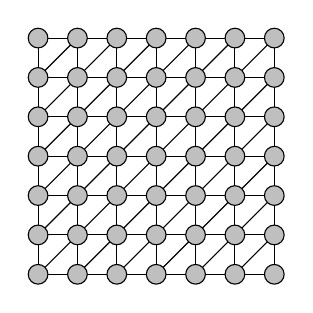
\begin{tikzpicture}[scale=.5]
\draw (0,0) grid (6,6);
\foreach \i in {0,...,5}
{
	\foreach \j in {0,...,5}
	{
		\draw (\i,\j) -- ({1+\i},{1+\j});
	}
}
\foreach \i in {0,...,6}
{
	\foreach \j in {0,...,6}
	{
		\draw[black,fill=gray!50] (\i,\j) circle (.25cm);
	}
}
\end{tikzpicture}
\]
The disks are the tiles.
Each tile has neighboring tiles at the corners of any small square it overlaps, and also across those squares on the diagonal lines.
Each interior tile has \(6\) neighbors, each edge tile \(4\) neighbors, the upper right and lower left corner tiles have \(3\) neighbors, and the upper left and lower right corner tiles have \(2\) neighbors.
Henceforth we only make use of this type of hex board; we leave the reader to work out how to turn one type of hex board into the other.
\begin{proof}
Our proof is by contradiction.
Each step leads to one fewer empty tile.
So if neither side wins, we can suppose that they keep playing until every tile on the board contains a stone, and yet somehow there is no path of white stones travelling from the left edge to the right, and no path of black stones from the top to the bottom.
Imagine that every disk, which we draw as gray, actually contains either a black or white stone, so should really be coloured either black or white.

We first add onto each side of the board a new row or column of tiles, of the same size as the board, so forming a square without its corners, with the diagonal lines, south west to north east, added at the two corners where that is possible (the upper left and lower right):
\[
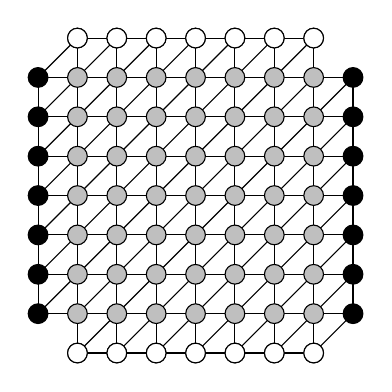
\begin{tikzpicture}[scale=.5]
\draw (-1,0) grid (7,6);
\draw (0,-1) grid (6,7);
\foreach \i in {-1,...,6}
{
	\foreach \j in {0,...,5}
	{
		\draw (\i,\j) -- ({1+\i},{1+\j});
	}
}
\foreach \i in {0,...,6}
{
\draw ({\i-1},6) -- (\i,7);
\draw (\i,-1) -- ({\i+1},0);
}
\foreach \i in {0,...,6}
{
	\foreach \j in {-1,...,7}
	{
		\draw[black,fill=gray!50] (\i,\j) circle (.25cm);
	}
	\draw[black,fill=white] (\i,-1) circle (.25cm);
	\draw[black,fill=white] (\i,7) circle (.25cm);
	\draw[black,fill=black] (-1,\i) circle (.25cm);
	\draw[black,fill=black] (7,\i) circle (.25cm);
}
\end{tikzpicture}
\]
We put black stones in all of the new left and right tiles, and white in all of the new top and bottom tiles.
Don't step on the stones, but only on the triangles; start at the lower right corner triangle:
\[
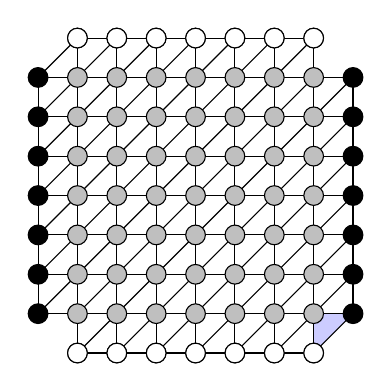
\begin{tikzpicture}[scale=.5]
\fill[blue!20] (6,-1) -- (7,0) -- (6,0) -- cycle;
\draw (-1,0) grid (7,6);
\draw (0,-1) grid (6,7);
\foreach \i in {-1,...,6}
{
	\foreach \j in {0,...,5}
	{
		\draw (\i,\j) -- ({1+\i},{1+\j});
	}
}
\foreach \i in {0,...,6}
{
\draw ({\i-1},6) -- (\i,7);
\draw (\i,-1) -- ({\i+1},0);
}
\foreach \i in {0,...,6}
{
	\foreach \j in {-1,...,7}
	{
		\draw[black,fill=gray!50] (\i,\j) circle (.25cm);
	}
	\draw[black,fill=white] (\i,-1) circle (.25cm);
	\draw[black,fill=white] (\i,7) circle (.25cm);
	\draw[black,fill=black] (-1,\i) circle (.25cm);
	\draw[black,fill=black] (7,\i) circle (.25cm);
}
\end{tikzpicture}
\]

An edge is \emph{mixed} if it has a white stone on one tile and a black stone on the other.
A triangle is \emph{mixed} if not all of its stones are the same colour, so it has a black stone on one corner and a white stone on another corner.
The third corner then has a black or white stone on it.
So every mixed triangle has two mixed edges and one edge not mixed.

Our first triangle is mixed: it has a white and black stone on the lower right edge.
So it has a second mixed edge.
Step over that edge to the next triangle.

Suppose inductively that we are on a mixed triangle, and we entered it via a mixed edge.
It has precisely one other mixed edge.
We have to step across that edge next.
So there is a uniquely determined sequence of triangles.
We always head across an edge, so we never step on the same triangle two times in a row, since no triangle is a neighbor of itself.

%import random
%for i in range(0,7):
%    for j in range(0,7):
%        n = random.randint(0,1)
%        if (n==0):
%            print("\\draw[black,fill=white] ({0},{1}) circle (.25cm);".format(i,j))
%        else:
%            print("\\draw[black,fill=black] ({0},{1}) circle (.25cm);".format(i,j))        

For example, if we start with:
\[
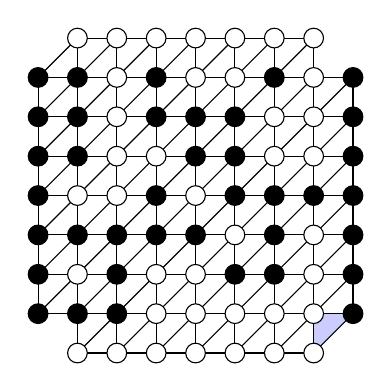
\begin{tikzpicture}[scale=.5]
\fill[blue!20] (6,-1) -- (7,0) -- (6,0) -- cycle;
\draw (-1,0) grid (7,6);
\draw (0,-1) grid (6,7);
\foreach \i in {-1,...,6}
{
	\foreach \j in {0,...,5}
	{
		\draw (\i,\j) -- ({1+\i},{1+\j});
	}
}
\foreach \i in {0,...,6}
{
\draw ({\i-1},6) -- (\i,7);
\draw (\i,-1) -- ({\i+1},0);
}
\foreach \i in {0,...,6}
{
	\draw[black,fill=white] (\i,-1) circle (.25cm);
	\draw[black,fill=white] (\i,7) circle (.25cm);
	\draw[black,fill=black] (-1,\i) circle (.25cm);
	\draw[black,fill=black] (7,\i) circle (.25cm);
}
\draw[black,fill=black] (0,0) circle (.25cm);
\draw[black,fill=white] (0,1) circle (.25cm);
\draw[black,fill=black] (0,2) circle (.25cm);
\draw[black,fill=white] (0,3) circle (.25cm);
\draw[black,fill=black] (0,4) circle (.25cm);
\draw[black,fill=black] (0,5) circle (.25cm);
\draw[black,fill=black] (0,6) circle (.25cm);
\draw[black,fill=black] (1,0) circle (.25cm);
\draw[black,fill=black] (1,1) circle (.25cm);
\draw[black,fill=black] (1,2) circle (.25cm);
\draw[black,fill=white] (1,3) circle (.25cm);
\draw[black,fill=white] (1,4) circle (.25cm);
\draw[black,fill=white] (1,5) circle (.25cm);
\draw[black,fill=white] (1,6) circle (.25cm);
\draw[black,fill=white] (2,0) circle (.25cm);
\draw[black,fill=white] (2,1) circle (.25cm);
\draw[black,fill=black] (2,2) circle (.25cm);
\draw[black,fill=black] (2,3) circle (.25cm);
\draw[black,fill=white] (2,4) circle (.25cm);
\draw[black,fill=black] (2,5) circle (.25cm);
\draw[black,fill=black] (2,6) circle (.25cm);
\draw[black,fill=white] (3,0) circle (.25cm);
\draw[black,fill=white] (3,1) circle (.25cm);
\draw[black,fill=black] (3,2) circle (.25cm);
\draw[black,fill=white] (3,3) circle (.25cm);
\draw[black,fill=black] (3,4) circle (.25cm);
\draw[black,fill=black] (3,5) circle (.25cm);
\draw[black,fill=white] (3,6) circle (.25cm);
\draw[black,fill=white] (4,0) circle (.25cm);
\draw[black,fill=black] (4,1) circle (.25cm);
\draw[black,fill=white] (4,2) circle (.25cm);
\draw[black,fill=black] (4,3) circle (.25cm);
\draw[black,fill=black] (4,4) circle (.25cm);
\draw[black,fill=black] (4,5) circle (.25cm);
\draw[black,fill=white] (4,6) circle (.25cm);
\draw[black,fill=white] (5,0) circle (.25cm);
\draw[black,fill=black] (5,1) circle (.25cm);
\draw[black,fill=black] (5,2) circle (.25cm);
\draw[black,fill=black] (5,3) circle (.25cm);
\draw[black,fill=white] (5,4) circle (.25cm);
\draw[black,fill=white] (5,5) circle (.25cm);
\draw[black,fill=black] (5,6) circle (.25cm);
\draw[black,fill=white] (6,0) circle (.25cm);
\draw[black,fill=white] (6,1) circle (.25cm);
\draw[black,fill=white] (6,2) circle (.25cm);
\draw[black,fill=black] (6,3) circle (.25cm);
\draw[black,fill=white] (6,4) circle (.25cm);
\draw[black,fill=white] (6,5) circle (.25cm);
\draw[black,fill=white] (6,6) circle (.25cm);
\end{tikzpicture}
\]
then our triangles are:
\[
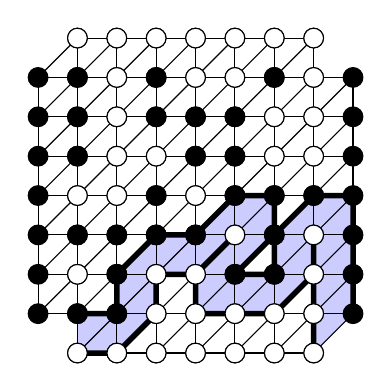
\begin{tikzpicture}[scale=.5]
\fill[blue!20] (6,-1) -- (7,0) -- (6,0) -- cycle;
\fill[blue!20] (6,0) -- (7,0) -- (7,1) -- cycle;
\fill[blue!20] (6,0) -- (7,1) -- (6,1) -- cycle;
\fill[blue!20] (6,1) -- (7,1) -- (7,2) -- cycle;
\fill[blue!20] (6,1) -- (7,2) -- (6,2) -- cycle;
\fill[blue!20] (6,2) -- (7,2) -- (7,3) -- cycle;
\fill[blue!20] (6,2) -- (7,3) -- (6,3) -- cycle;
\fill[blue!20] (5,2) -- (6,2) -- (6,3) -- cycle;
\fill[blue!20] (5,1) -- (6,2) -- (5,2) -- cycle;
\fill[blue!20] (5,1) -- (6,1) -- (6,2) -- cycle;
\fill[blue!20] (5,0) -- (6,1) -- (5,1) -- cycle;
\fill[blue!20] (4,0) -- (5,0) -- (5,1) -- cycle;
\fill[blue!20] (4,0) -- (5,1) -- (4,1) -- cycle;
\fill[blue!20] (3,0) -- (4,0) -- (4,1) -- cycle;
\fill[blue!20] (3,0) -- (4,1) -- (3,1) -- cycle;
\fill[blue!20] (3,1) -- (4,1) -- (4,2) -- cycle;
\fill[blue!20] (4,1) -- (5,2) -- (4,2) -- cycle;
\fill[blue!20] (4,2) -- (5,2) -- (5,3) -- cycle;
\fill[blue!20] (4,2) -- (5,3) -- (4,3) -- cycle;
\fill[blue!20] (3,2) -- (4,2) -- (4,3) -- cycle;
\fill[blue!20] (3,1) -- (4,2) -- (3,2) -- cycle;
\fill[blue!20] (2,1) -- (3,1) -- (3,2) -- cycle;
\fill[blue!20] (2,1) -- (3,2) -- (2,2) -- cycle;
\fill[blue!20] (1,1) -- (2,1) -- (2,2) -- cycle;
\fill[blue!20] (1,0) -- (2,1) -- (1,1) -- cycle;
\fill[blue!20] (1,0) -- (2,0) -- (2,1) -- cycle;
\fill[blue!20] (1,-1) -- (2,0) -- (1,0) -- cycle;
\fill[blue!20] (0,-1) -- (1,-1) -- (1,0) -- cycle;
\fill[blue!20] (0,-1) -- (1,0) -- (0,0) -- cycle;
\draw (-1,0) grid (7,6);
\draw (0,-1) grid (6,7);
\draw[line width=2pt] (6,-1) -- (6,2) -- (6,1) -- (5,0) -- (3,0) -- (3,1) -- (4,2) -- (3,1) -- (2,1) -- (2,0) -- (1,-1) -- (0,-1);
\draw[line width=2pt] (7,0) -- (7,3) -- (6,3) -- (5,2) -- (5,1) -- (4,1) -- (5,2) -- (5,3) -- (4,3) -- (3,2) -- (2,2) -- (1,1) -- (1,0) -- (0,0);
\foreach \i in {-1,...,6}
{
	\foreach \j in {0,...,5}
	{
		\draw (\i,\j) -- ({1+\i},{1+\j});
	}
}
\foreach \i in {0,...,6}
{
\draw ({\i-1},6) -- (\i,7);
\draw (\i,-1) -- ({\i+1},0);
}
\foreach \i in {0,...,6}
{
	\foreach \j in {-1,...,7}
	{
		\draw[black,fill=gray!50] (\i,\j) circle (.25cm);
	}
	\draw[black,fill=white] (\i,-1) circle (.25cm);
	\draw[black,fill=white] (\i,7) circle (.25cm);
	\draw[black,fill=black] (-1,\i) circle (.25cm);
	\draw[black,fill=black] (7,\i) circle (.25cm);
}
\draw[black,fill=black] (0,0) circle (.25cm);
\draw[black,fill=white] (0,1) circle (.25cm);
\draw[black,fill=black] (0,2) circle (.25cm);
\draw[black,fill=white] (0,3) circle (.25cm);
\draw[black,fill=black] (0,4) circle (.25cm);
\draw[black,fill=black] (0,5) circle (.25cm);
\draw[black,fill=black] (0,6) circle (.25cm);
\draw[black,fill=black] (1,0) circle (.25cm);
\draw[black,fill=black] (1,1) circle (.25cm);
\draw[black,fill=black] (1,2) circle (.25cm);
\draw[black,fill=white] (1,3) circle (.25cm);
\draw[black,fill=white] (1,4) circle (.25cm);
\draw[black,fill=white] (1,5) circle (.25cm);
\draw[black,fill=white] (1,6) circle (.25cm);
\draw[black,fill=white] (2,0) circle (.25cm);
\draw[black,fill=white] (2,1) circle (.25cm);
\draw[black,fill=black] (2,2) circle (.25cm);
\draw[black,fill=black] (2,3) circle (.25cm);
\draw[black,fill=white] (2,4) circle (.25cm);
\draw[black,fill=black] (2,5) circle (.25cm);
\draw[black,fill=black] (2,6) circle (.25cm);
\draw[black,fill=white] (3,0) circle (.25cm);
\draw[black,fill=white] (3,1) circle (.25cm);
\draw[black,fill=black] (3,2) circle (.25cm);
\draw[black,fill=white] (3,3) circle (.25cm);
\draw[black,fill=black] (3,4) circle (.25cm);
\draw[black,fill=black] (3,5) circle (.25cm);
\draw[black,fill=white] (3,6) circle (.25cm);
\draw[black,fill=white] (4,0) circle (.25cm);
\draw[black,fill=black] (4,1) circle (.25cm);
\draw[black,fill=white] (4,2) circle (.25cm);
\draw[black,fill=black] (4,3) circle (.25cm);
\draw[black,fill=black] (4,4) circle (.25cm);
\draw[black,fill=black] (4,5) circle (.25cm);
\draw[black,fill=white] (4,6) circle (.25cm);
\draw[black,fill=white] (5,0) circle (.25cm);
\draw[black,fill=black] (5,1) circle (.25cm);
\draw[black,fill=black] (5,2) circle (.25cm);
\draw[black,fill=black] (5,3) circle (.25cm);
\draw[black,fill=white] (5,4) circle (.25cm);
\draw[black,fill=white] (5,5) circle (.25cm);
\draw[black,fill=black] (5,6) circle (.25cm);
\draw[black,fill=white] (6,0) circle (.25cm);
\draw[black,fill=white] (6,1) circle (.25cm);
\draw[black,fill=white] (6,2) circle (.25cm);
\draw[black,fill=black] (6,3) circle (.25cm);
\draw[black,fill=white] (6,4) circle (.25cm);
\draw[black,fill=white] (6,5) circle (.25cm);
\draw[black,fill=white] (6,6) circle (.25cm);
\end{tikzpicture}
\]
We see that we start at one corner and end at another.
The stones on our right hand side are black, and on our left hand side are right.

We want to see that we never step on triangle twice.
Suppose that this sequence of triangles enters a loop sometime after the first step.
Let \(B\) be the first triangle we encounter for a second time.
The first time we reach \(B\), we come from some triangle \(A\), and leave to some triangle \(C\), so our path is \(\dots ABC\dots\).
The second time we reach \(B\), we come across one mixed edge and then leave across another.
But triangles \(A\) and \(C\) are across those edges.
So we must travel \(\dots ABC\dots ABC\dots\) or \(\dots ABC\dots CBA\dots\).
In the first case, \(B\) is not the first triangle we hit twice: we already hit \(A\) twice previously.
In the second case, \(B\) is not the first triangle we hit twice: we already hit \(C\) twice previously.

So if there is a loop, the first repetition is at the first triangle, where we entered:
\[
AB\dots A\dots 
\]
But there is only one mixed edge of \(A\) we can cross through, and we step across it when we reach \(B\).
We must therefore pass across that same edge when we get back to \(A\) again:
\[
AB\dots BA\dots 
\]
Again a contradiction: \(A\) is not the first triangle we reach for a second time.

Since there is no loop in our path of triangles, our path ends.
But we can keep stepping until we reach a triangle whose mixed edge doesn't lead to another triangle.
These can only be triangles at the corners (and even some of them might not be mixed edges): 
\[
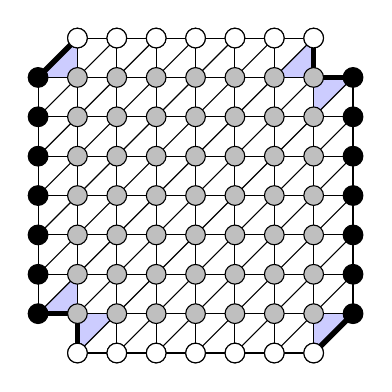
\begin{tikzpicture}[scale=.5]
\fill[blue!20] (6,-1) -- (7,0) -- (6,0) -- cycle;
\draw[line width=2pt] (6,-1) -- (7,0);
\fill[blue!20] (-1,6) -- (0,7) -- (0,6) -- cycle;
\draw[line width=2pt] (-1,6) -- (0,7);
\fill[blue!20] (0,-1) -- (1,0) -- (0,0) -- cycle;
\draw[line width=2pt] (0,-1) -- (0,0);
\fill[blue!20] (-1,0) -- (0,1) -- (0,0) -- cycle;
\draw[line width=2pt] (-1,0) -- (0,0);
\fill[blue!20] (6,6) -- (6,7) -- (5,6) -- cycle;
\draw[line width=2pt] (6,6) -- (6,7);
\fill[blue!20] (6,6) -- (7,6) -- (6,5) -- cycle;
\draw[line width=2pt] (6,6) -- (7,6);
\draw (-1,0) grid (7,6);
\draw (0,-1) grid (6,7);
\foreach \i in {-1,...,6}
{
	\foreach \j in {0,...,5}
	{
		\draw (\i,\j) -- ({1+\i},{1+\j});
	}
}
\foreach \i in {0,...,6}
{
\draw ({\i-1},6) -- (\i,7);
\draw (\i,-1) -- ({\i+1},0);
}
\foreach \i in {0,...,6}
{
	\foreach \j in {-1,...,7}
	{
		\draw[black,fill=gray!50] (\i,\j) circle (.25cm);
	}
	\draw[black,fill=white] (\i,-1) circle (.25cm);
	\draw[black,fill=white] (\i,7) circle (.25cm);
	\draw[black,fill=black] (-1,\i) circle (.25cm);
	\draw[black,fill=black] (7,\i) circle (.25cm);
}
\end{tikzpicture}
\]
Since there is no loop, we reach a corner which is not the one we started at.

We started with a black stone on our right, and kept having a black stone on our right at every step.
If we end up at the opposite corner, then we end up with a black stone on our right, impossible.
\[
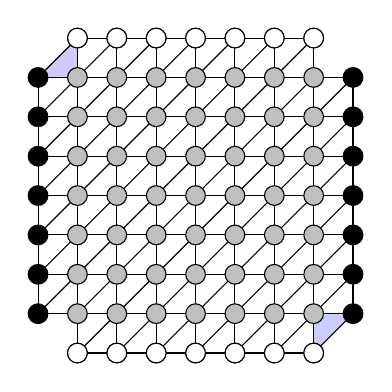
\begin{tikzpicture}[scale=.5]
\fill[blue!20] (6,-1) -- (7,0) -- (6,0) -- cycle;
\fill[blue!20] (-1,6) -- (0,7) -- (0,6) -- cycle;
\draw (-1,0) grid (7,6);
\draw (0,-1) grid (6,7);
\foreach \i in {-1,...,6}
{
	\foreach \j in {0,...,5}
	{
		\draw (\i,\j) -- ({1+\i},{1+\j});
	}
}
\foreach \i in {0,...,6}
{
\draw ({\i-1},6) -- (\i,7);
\draw (\i,-1) -- ({\i+1},0);
}
\foreach \i in {0,...,6}
{
	\foreach \j in {-1,...,7}
	{
		\draw[black,fill=gray!50] (\i,\j) circle (.25cm);
	}
	\draw[black,fill=white] (\i,-1) circle (.25cm);
	\draw[black,fill=white] (\i,7) circle (.25cm);
	\draw[black,fill=black] (-1,\i) circle (.25cm);
	\draw[black,fill=black] (7,\i) circle (.25cm);
}
\end{tikzpicture}
\]
So we end up at one of the other two corners, in one of its two neighboring triangles.
In these triangles, the four edges indicated here may or may not be mixed.
\[
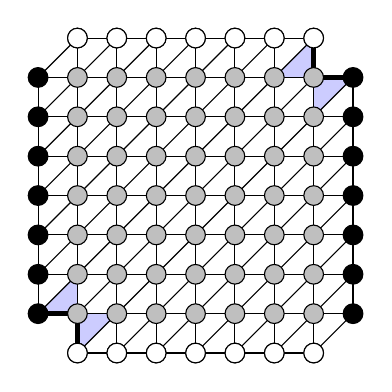
\begin{tikzpicture}[scale=.5]
\fill[blue!20] (0,-1) -- (1,0) -- (0,0) -- cycle;
\draw[line width=2pt] (0,-1) -- (0,0);
\fill[blue!20] (-1,0) -- (0,1) -- (0,0) -- cycle;
\draw[line width=2pt] (-1,0) -- (0,0);
\fill[blue!20] (6,6) -- (6,7) -- (5,6) -- cycle;
\draw[line width=2pt] (6,6) -- (6,7);
\fill[blue!20] (6,6) -- (7,6) -- (6,5) -- cycle;
\draw[line width=2pt] (6,6) -- (7,6);
\draw (-1,0) grid (7,6);
\draw (0,-1) grid (6,7);
\foreach \i in {-1,...,6}
{
	\foreach \j in {0,...,5}
	{
		\draw (\i,\j) -- ({1+\i},{1+\j});
	}
}
\foreach \i in {0,...,6}
{
\draw ({\i-1},6) -- (\i,7);
\draw (\i,-1) -- ({\i+1},0);
}
\foreach \i in {0,...,6}
{
	\foreach \j in {-1,...,7}
	{
		\draw[black,fill=gray!50] (\i,\j) circle (.25cm);
	}
	\draw[black,fill=white] (\i,-1) circle (.25cm);
	\draw[black,fill=white] (\i,7) circle (.25cm);
	\draw[black,fill=black] (-1,\i) circle (.25cm);
	\draw[black,fill=black] (7,\i) circle (.25cm);
}
\end{tikzpicture}
\]

As we travel, we have a black stone to our right, and a white stone to our left, at every step.
Hence a path of black stones to our right, and a path of white stones to our left.
One of these paths meets the corner tile, a winning path.
\end{proof}
There is an \(n\)-dimensional \(n\)-player version of hex, but it is too complicated to describe here.
\section{Vector fields}
\begin{center}
\includegraphics[width=8cm]{AN-Leonardo-Water-Study-723926.jpg}
\legend{Leonardo da~Vinci, \emph{Study of water falling into still water}, c. 1508-9}
\end{center}
Let \(X=[0,1]\times [0,1]\).
A \emph{vector field} \(v\) on \(X\) is a continuous map \(X\xrightarrow{v}\R{2}\).
Picture the vector field as the velocity of a flowing fluid.
We are particularly interested in the points where the vector field vanishes, so a little particle of the fluid does not move.
A vector field is \emph{inward}\define{inward} (or perhaps we should say \emph{not outward}) if the fluid can flow in, but doesn't flow out, of the square \(X\), i.e.\ at each point \(p=(x,y)\in X\), the vector \(v(p)\) doesn't point to the left along the left side, doesn't point up along the top, and so on.
To be more precise, if \(v(p)=(\xi(x,y),\eta(x,y))\), we require that
\begin{align*}
\xi(0,y)&\ge 0 \text{ for all } 0\le y\le 1,\\
\xi(1,y)&\le 0 \text{ for all } 0\le y\le 1,\\
\eta(x,0)&\ge 0 \text{ for all } 0\le x\le 1,\\
\eta(x,1)&\le 0 \text{ for all } 0\le x\le 1.
\end{align*}
A vector field \(v\) is \emph{outward}\define{outward} if \(-v\) is inward.
\begin{theorem}
Every inward or outward vector field on a square vanishes at some point of the square.
\end{theorem}
\begin{proof}
It is enough to prove for inward vector fields, since any outward field \(v\) vanishes just where \(-v\) vanishes.
We can suppose that our square is the unit square \(X=[0,1]\times[0,1]\) and denote our vector field
\[
X\xrightarrow{v}\R{2}.
\]

Suppose that \(v\) has no zero in \(X\), so every point \(p\in X\), \(v(p)\ne 0\).
By compactness of \(X\), we can find some point of \(X\) where \(|v|\) acheives its infimum length, so there is a positive lower bound on \(|v|\), so ther is some \(\varepsilon>0\) so that
\[
|v(p)|>\sqrt{2}\varepsilon>0
\]
for all \(p\in X\).
The reason for putting in a factor of \(\sqrt{2}\) here is that at least one entry of the vector is larger than \(\varepsilon\) in absolute value; to see this, write the entries of \(v\), say \(v(p)=(\xi,\eta)\) and then
\[
\xi^2+\eta^2=|v(p)|^2>2\varepsilon^2,
\]
so at least one of \(\xi^2,\eta^2\) is larger than \(\varepsilon^2\), so at least one of \(|\xi|,|\eta|\) is larger than \(\varepsilon\).

The square \(X\) is compact and \(v\) is continuous, hence \(v\) is uniformly continuous.
By uniform continuity, there is some \(\delta>0\) so that if \(p,q\in X\) have \(|p-q|<\delta\)  then \(|v(p)-v(q)|<\varepsilon\).
Pick some integer \(n\) larger than \(\sqrt{2}/\delta\), so
\[
0<\frac{1}{n}<\frac{\delta}{\sqrt{2}}.
\]

Divide \(X\) into an \(n\times n\) square hex board with small squares of length and height \(1/n\) each.
The center \(p\) of any tile has at least one of \(\xi(p),\eta(p)\) larger than \(\varepsilon\) in absolute value.
Put a white stone on the tile with center \(p\) if \(|\xi(p)|<|\eta(p)|\), i.e. if \(v(p)\) is ``mostly'' pointing up or down, and a black stone otherwise.
We want to see that this hex game has no winner.

Suppose we find a black stone on a tile with center \(p\in X\).
Since the stone is black, \(|\xi(p)|\ge|\eta(p)|\) and so \(|\xi(p)|>\varepsilon\).
We could ask whether \(\xi(p)>\varepsilon\) or whether instead \(\xi(p)<-\varepsilon\), a ``rightward'' or ``leftward'' black stone, i.e. with vector pointing ``mostly'' to the right or to the left.

Claim: if \(p\) and \(q\) are neighboring black stones, we can't have \(p\) rightward, and \(q\) leftward, i.e. we can't have both \(\xi(p)>\varepsilon\) and \(\xi(q)<-\varepsilon\).
Proof: suppose we did.
Because \(p\) and \(q\) are neighbors, they are of distance at most \(\sqrt{2}/n<\delta\), so
\begin{align*}
\varepsilon&>
|v(p)-v(q)|,\\
&\ge
|\xi(p)-\xi(q)|,
\\
&\ge 2\varepsilon
\end{align*}

Using the obvious analogous definitions, an upward white stone upward can't neighbor a downward white stone.
 
Take a path of black stones travelling from left to right.
On the left edge of the square \(X\), \(v\) does not point leftward, so each tile either has a white stone or else \(v\) is rightward and the stone is black.
On the right edge, the vector field does not point rightward, so each tile either has a white stone or \(v\) is leftward and the stone is black.
So our path starts rightward, ends leftward, and so contains a first step from a rightward to a leftward, black stones on neighboring tiles, a contradiction.

The same argument works for a path of white stones travelling from bottom to top.
We conclude that there is no winner in this game of hex, contradicting theorem~\vref{theorem:hex.has.a.winner}.
So finally we contradict our hypothesis that \(v\) vanishes nowhere.
So \(v\) vanishes somewhere.
\end{proof}
The \(n\)-player version of hex proves a similar theorem on the \(n\)-dimensional box, but the notation is too complicated to describe here.
\section{The Brouwer fixed point theorem}
\begin{theorem}[The Brouwer fixed point theorem]
Every continuous map of a square to itself fixes some point of the square.
\end{theorem}
Take two identical pieces of paper%
\SubIndex{paper}
of the same size and shape, one lying directly on top of the other.
Pick up the top piece of paper and crumple it. 
Put it on top of the other piece of paper, so that every point of the crumpled sheet lies above some point of the flat sheet.
Some point of the crumpled piece of paper is now lying exactly on top of the same point of the flat sheet which it was lying on before it was crumpled.
\begin{proof}
We can suppose that our square is the unit square \(X=[0,1]\times[0,1]\) and denote our map
\[
X\xrightarrow{\varphi}X.
\]
The \emph{error vector} of a point \(p=(x,y)\in X\) is \(v_p:=\varphi(p)-p\).
A fixed point is precisely a point \(p\in X\) where \(\varphi(p)=p\), i.e. with vanishing error vector \(v_p=0\).
Each point \(p\) moves under \(\varphi\) to the point \(p+v_p\), i.e. by adding its error vector.
Since no point is carried by \(\varphi\) off of the square, the vector field \(v\) is inward, so has a zero.
\end{proof}
\begin{problem}{brouwer.homeo}
Suppose that \(X\) is a topological space which is homeomorphic to a square.
Prove that every continuous map \(X\to X\) has a fixed point.
\end{problem}
The \(n\)-player version of hex proves a similar theorem on the \(n\)-dimensional box, but the notation is too complicated to describe here.

